\section{Results}
All numbers below come from \texttt{results/runs.csv} and \texttt{results/raw\_measurements.csv} through \texttt{scripts/analyze.py}.
Times are medians of the measured samples, with the relative IQR (IQR/median) in parentheses.

\subsection{Correctness, thread counts and campaign conditions}
The campaign ran 110 processes in 21~minutes (start times 19:47:59--20:08:41 UTC, 12 Nov.~2026) and collected 542 measured samples. All
110 processes finished with status \texttt{ok}; no budget was reached, so the \textbf{largest attempted and largest feasible size is
$n=4000$} (19.6~s per sequential multiplication, 367~MiB). Every product passed the NumPy check (largest relative error
$8.5\times10^{-15}$, below $2\gamma_n$) and \textbf{all 110 products were bit-identical to the sequential baseline} of the same $n$,
including every thread count, tile size and vector build. In all 88 \texttt{omp} processes the OpenMP team size and the number of
distinct OS threads that executed it were equal to the requested $p$. \texttt{CPU\_Speed\_Limit} was 100 before and after every
process (the OS never requested thermal throttling). The correctness suite (1404 checks: 351 on each of four binaries) reported no failure.

\subsection{Runtime}
Table~\ref{tab:time} and Fig.~\ref{fig:runtime} give the time per multiplication. The sequential baseline sustains 5.7--6.6~GFLOP/s
($2n^3/T$) for all sizes, so its time grows as $n^3$ (a factor 62\,200 from $n=100$ to $4000$ for a factor $64\,000$ in $n^3$). The parallel
version follows the same cubic trend shifted down by the speedup; four threads take 0.089~ms at $n=100$ and 5.75~s at $n=4000$.
Variability within a process was small: relative IQRs were below 9\% in 56 of the 60 configurations; the four larger ones (13--28\%) are $p=3$ at $n=100$, $p=8$ and $16$ at
$n=250$, and $p=8$ at $n=2000$.

\begin{table}[!htb]\centering\footnotesize\setlength{\tabcolsep}{3pt}
\caption{Time per multiplication, median (relative IQR) of 5 measured samples (3 at $n=4000$); campaigns \texttt{main} and \texttt{large}.
Batches of 607, 39 and 5 multiplications for $n=100,250,500$. ``--'': not planned. $p=16$ is oversubscribed (8 hardware threads).}
\label{tab:time}\resizebox{\linewidth}{!}{\begin{tabular}{rllllllll}
\toprule
$n$ & seq & $p{=}1$ & $p{=}2$ & $p{=}3$ & $p{=}4$ & $p{=}6$ & $p{=}8$ & $p{=}16$ \\
\midrule
100 & 0.314 ms\,(7.4\%) & 0.295 ms\,(0.57\%) & 0.151 ms\,(3.4\%) & 0.105 ms\,(16\%) & 0.0888 ms\,(8.0\%) & 0.0957 ms\,(4.3\%) & 0.0863 ms\,(5.3\%) & 0.117 ms\,(2.1\%) \\
250 & 4.73 ms\,(0.96\%) & 4.72 ms\,(0.76\%) & 2.48 ms\,(5.0\%) & 1.64 ms\,(1.5\%) & 1.33 ms\,(8.9\%) & 1.45 ms\,(0.44\%) & 1.56 ms\,(28\%) & 1.19 ms\,(24\%) \\
500 & 40.0 ms\,(0.66\%) & 39.7 ms\,(2.7\%) & 19.9 ms\,(1.0\%) & 13.5 ms\,(0.89\%) & 10.6 ms\,(6.9\%) & 11.6 ms\,(2.6\%) & 10.5 ms\,(2.3\%) & 10.3 ms\,(3.3\%) \\
1000 & 320 ms\,(0.40\%) & 319 ms\,(0.98\%) & 164 ms\,(3.3\%) & 108 ms\,(0.60\%) & 86.0 ms\,(2.8\%) & 90.1 ms\,(8.2\%) & 81.4 ms\,(1.6\%) & 84.8 ms\,(8.0\%) \\
1500 & 1.18 s\,(5.0\%) & 1.10 s\,(1.6\%) & 553 ms\,(0.38\%) & 371 ms\,(0.87\%) & 298 ms\,(1.9\%) & 298 ms\,(3.2\%) & 281 ms\,(0.78\%) & 282 ms\,(1.7\%) \\
2000 & 2.64 s\,(4.2\%) & 2.68 s\,(0.89\%) & 1.41 s\,(6.4\%) & 932 ms\,(8.5\%) & 755 ms\,(6.2\%) & 729 ms\,(2.5\%) & 744 ms\,(13\%) & 782 ms\,(3.0\%) \\
3000 & 8.57 s\,(1.2\%) & 8.32 s\,(0.64\%) & 4.32 s\,(1.3\%) & 3.05 s\,(2.8\%) & 2.39 s\,(1.1\%) & 2.45 s\,(1.8\%) & 2.41 s\,(2.9\%) & 2.30 s\,(0.31\%) \\
4000 & 19.6 s\,(0.52\%) & 19.5 s\,(0.66\%) & -- & -- & 5.75 s\,(2.1\%) & -- & 5.55 s\,(1.8\%) & -- \\
\bottomrule
\end{tabular}
}
\end{table}

\begin{figure}[!htb]\centering
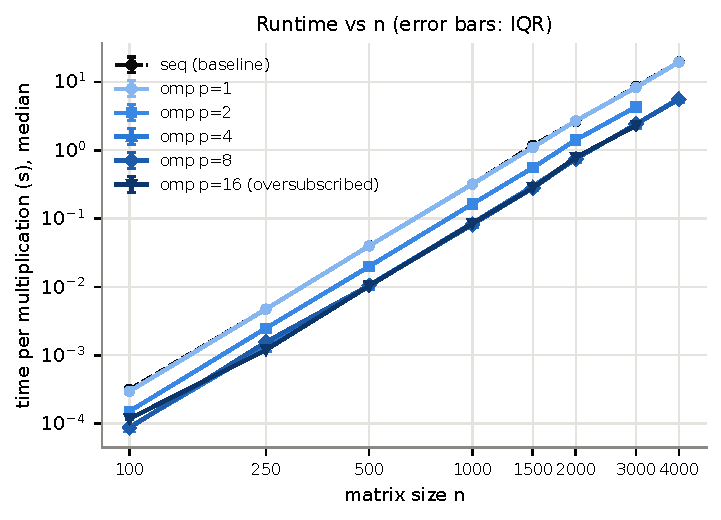
\includegraphics[width=0.62\linewidth]{fig1_runtime}
\caption{Median time per multiplication against $n$ (log--log) for the sequential baseline and selected thread counts; error bars are the IQR (mostly hidden by the markers).}
\label{fig:runtime}
\end{figure}

\subsection{Speedup and efficiency}
Table~\ref{tab:speedup} and Figs.~\ref{fig:speedup}--\ref{fig:svsn} show $S(p)=T_{seq}/T_p$ and $E(p)=S(p)/p$ from medians.
\begin{itemize}
\item \textbf{Up to the physical cores.} $S(2)=1.87$--$2.13$, $S(3)=2.81$--$3.17$ and $S(4)=3.40$--$3.95$ for every $n$; $E(4)=0.85$--$0.99$.
\item \textbf{Beyond 4 threads.} Using the 8 hardware threads changes the speedup by a factor $S(8)/S(4)=0.85$--$1.06$ (Table~\ref{tab:best}); for
$n\ge500$ the change is $-1\%$ to $+6\%$. $E(8)=0.38$--$0.52$. $p=6$ is never more than $2\%$ better than the better of $p=4$ and $p=8$.
\item \textbf{Oversubscription.} $S(16)/S(8)=0.74$--$1.31$: no systematic gain; clear loss only at $n=100$ ($-26\%$); the $+31\%$ at $n=250$ coincides with
relative IQRs of 24--28\% for $p=8$ and $p=16$.
\item \textbf{Best configuration.} The highest median speedup per size is 3.52--4.19, reached with $p\in\{6,8,16\}$, but always within $7\%$ of $S(4)$
except at $n=250$ (11\%, noisy).
\item \textbf{Small sizes.} Even at $n=100$, where one sequential multiplication takes 0.31~ms, four threads give $S=3.54$ (IQR range 3.27--3.84).
No tested size has $S(p)<1$ for any $p\ge2$ (Fig.~\ref{fig:svsn}).
\end{itemize}

\begin{table}[!htb]\centering\footnotesize
\caption{Speedup / efficiency, $S(p)=T_{seq}/T_p$ and $E(p)=S(p)/p$, from medians.}
\label{tab:speedup}\begin{tabular}{rccccccc}
\toprule
$n$ & $p{=}1$ & $p{=}2$ & $p{=}3$ & $p{=}4$ & $p{=}6$ & $p{=}8$ & $p{=}16$ \\
\midrule
100 & 1.06 / 1.06 & 2.08 / 1.04 & 2.99 / 1.00 & 3.54 / 0.89 & 3.28 / 0.55 & 3.64 / 0.46 & 2.68 / 0.17 \\
250 & 1.00 / 1.00 & 1.90 / 0.95 & 2.89 / 0.96 & 3.56 / 0.89 & 3.25 / 0.54 & 3.03 / 0.38 & 3.96 / 0.25 \\
500 & 1.01 / 1.01 & 2.01 / 1.00 & 2.95 / 0.98 & 3.77 / 0.94 & 3.45 / 0.58 & 3.81 / 0.48 & 3.87 / 0.24 \\
1000 & 1.00 / 1.00 & 1.95 / 0.98 & 2.97 / 0.99 & 3.72 / 0.93 & 3.55 / 0.59 & 3.93 / 0.49 & 3.77 / 0.24 \\
1500 & 1.07 / 1.07 & 2.13 / 1.06 & 3.17 / 1.06 & 3.95 / 0.99 & 3.95 / 0.66 & 4.19 / 0.52 & 4.17 / 0.26 \\
2000 & 0.98 / 0.98 & 1.87 / 0.94 & 2.83 / 0.94 & 3.50 / 0.87 & 3.62 / 0.60 & 3.55 / 0.44 & 3.38 / 0.21 \\
3000 & 1.03 / 1.03 & 1.99 / 0.99 & 2.81 / 0.94 & 3.59 / 0.90 & 3.50 / 0.58 & 3.55 / 0.44 & 3.73 / 0.23 \\
4000 & 1.00 / 1.00 & -- & -- & 3.40 / 0.85 & -- & 3.52 / 0.44 & -- \\
\bottomrule
\end{tabular}

\end{table}

\begin{figure}[!htb]\centering
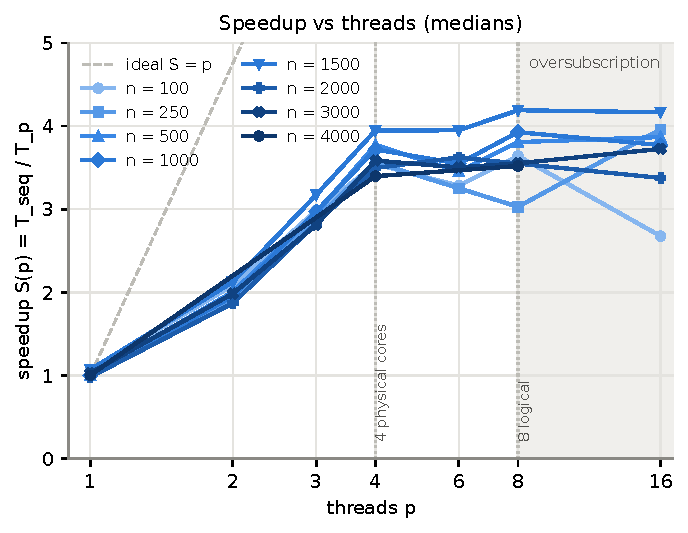
\includegraphics[width=0.49\linewidth]{fig2_speedup}\hfill
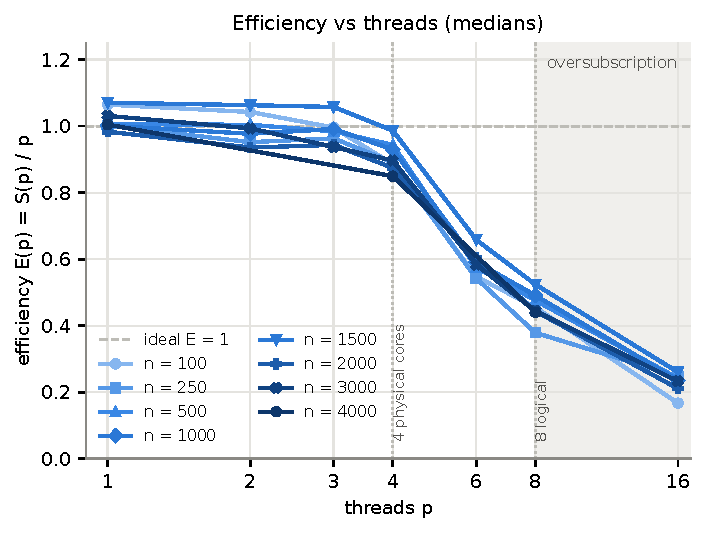
\includegraphics[width=0.49\linewidth]{fig3_efficiency}
\caption{Speedup (left) and efficiency (right) against the number of threads, one line per $n$ (darker = larger). Dashed: ideal. Dotted: 4 physical cores and 8 logical processors; shaded: oversubscription.}
\label{fig:speedup}
\end{figure}

\begin{figure}[!htb]\centering
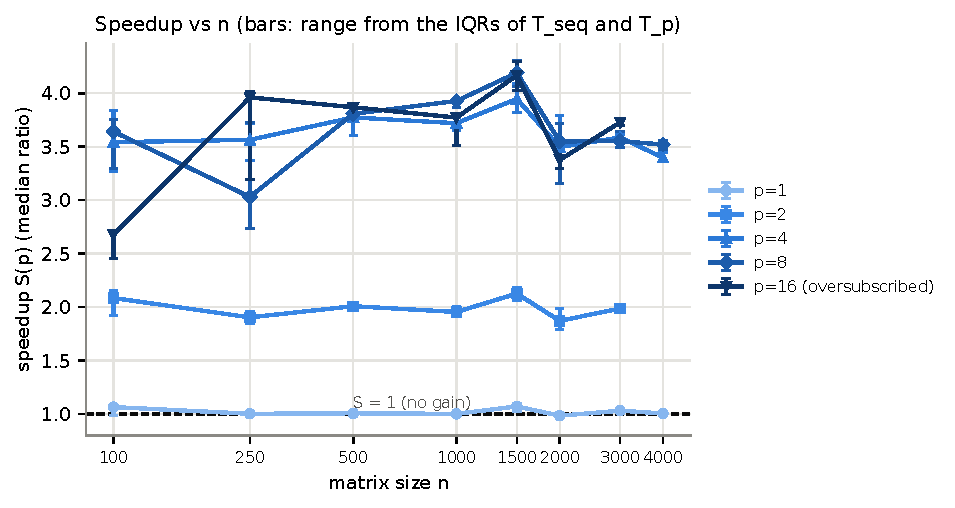
\includegraphics[width=0.6\linewidth]{fig4_speedup_vs_n}
\caption{Speedup against $n$ for selected $p$. Bars: rough range $[Q_1(T_{seq})/Q_3(T_p),\,Q_3(T_{seq})/Q_1(T_p)]$.}
\label{fig:svsn}
\end{figure}

\begin{table}[!htb]\centering\footnotesize
\caption{Best median speedup per size, its IQR-based range and efficiency, and the effect of Hyper-Threading ($S(8)/S(4)$) and oversubscription ($S(16)/S(8)$).}
\label{tab:best}\begin{tabular}{rrllll}
\toprule
$n$ & best $p$ & $S$ (IQR range) & $E$ & $S(8)/S(4)$ & $S(16)/S(8)$ \\
\midrule
100 & 8 & 3.64 (3.30--3.76) & 0.46 & 1.03 & 0.735 \\
250 & 16 & 3.96 (3.19--4.01) & 0.25 & 0.850 & 1.31 \\
500 & 16 & 3.87 (3.75--3.90) & 0.24 & 1.01 & 1.02 \\
1000 & 8 & 3.93 (3.87--3.95) & 0.49 & 1.06 & 0.960 \\
1500 & 8 & 4.19 (4.06--4.30) & 0.52 & 1.06 & 0.994 \\
2000 & 6 & 3.62 (3.56--3.81) & 0.60 & 1.02 & 0.951 \\
3000 & 16 & 3.73 (3.70--3.75) & 0.23 & 0.991 & 1.05 \\
4000 & 8 & 3.52 (3.48--3.56) & 0.44 & 1.04 & -- \\
\bottomrule
\end{tabular}

\end{table}

\textbf{Apparent superlinear values.} $E>1$ appears at $n=1500$ ($E(2)=1.06$, $E(3)=1.06$), $n=100$ ($E(2)=1.04$) and for $p=1$ at
$n=100$, $1500$ and $3000$ ($S(1)=1.03$--$1.07$). They are not taken at face value: in each case the parallel run with \emph{one} thread---the
same instructions on one core---is also faster than the sequential run (Table~\ref{tab:overhead}). Measured against the one-thread parallel
run, $S_1(p)=T_{omp,1}/T_p$, the efficiencies are at most 1.00 for every $n$ and $p$: at $n=1500$, $S_1(2)=1.99$, $S_1(3)=2.96$, $S_1(4)=3.69$; at $n=100$,
$S_1(2)=1.96$. The cause is therefore a slower sequential process at those sizes (between-process variability, Section~\ref{sec:var}), not a
cache effect of the parallel version; the sequential runs at $n=100$ and $n=1500$ also have the two largest relative IQRs among the sequential runs (7.4\% and 5.0\%).

\subsection{Overhead of the parallel version with one thread}
Table~\ref{tab:overhead} compares \texttt{omp} with $p=1$ against \texttt{seq}. The ratio is within $\pm5\%$ for six of the eight sizes
(0.970--1.017) and below $0.95$ at $n=100$ (0.939) and $n=1500$ (0.934), where the \emph{parallel} run is the faster one. No positive overhead of
the OpenMP region larger than $2\%$ is visible at any size.

\begin{table}[!htb]\centering\footnotesize
\caption{Parallel version with one thread vs.\ sequential baseline: median (IQR) and ratio of medians.}
\label{tab:overhead}\begin{tabular}{rlll}
\toprule
$n$ & $T_{seq}$ (IQR) & $T_{omp,1}$ (IQR) & $T_{omp,1}/T_{seq}$ \\
\midrule
100 & 0.314 ms (0.0233 ms) & 0.295 ms (0.00170 ms) & 0.939 \\
250 & 4.73 ms (0.0454 ms) & 4.72 ms (0.0357 ms) & 0.998 \\
500 & 40.0 ms (0.265 ms) & 39.7 ms (1.06 ms) & 0.994 \\
1000 & 320 ms (1.29 ms) & 319 ms (3.14 ms) & 0.999 \\
1500 & 1.18 s (58.7 ms) & 1.10 s (17.2 ms) & 0.934 \\
2000 & 2.64 s (110 ms) & 2.68 s (24.0 ms) & 1.02 \\
3000 & 8.57 s (102 ms) & 8.32 s (53.6 ms) & 0.970 \\
4000 & 19.6 s (102 ms) & 19.5 s (129 ms) & 0.995 \\
\bottomrule
\end{tabular}

\end{table}

\subsection{Memory}
Peak resident memory (\texttt{ru\_maxrss}) is the array storage $3\cdot8n^2$ plus a small constant: 0.7--0.8~MiB above it for the sequential
process and 0.4--0.6~MiB more for any parallel process (Table~\ref{tab:mem}, Fig.~\ref{fig:mem}). Across thread counts at a fixed $n$, the parallel
values differ by at most 0.34~MiB (at $n=100$, between $p=1$ and $p=16$), i.e.\ memory does not grow with $p$ beyond thread stacks and runtime
structures.

\begin{table}[!htb]\centering\footnotesize
\caption{Peak resident set size (MiB, \texttt{getrusage} \texttt{ru\_maxrss}, bytes on macOS) against the array storage $3\cdot 8n^2$.}
\label{tab:mem}\begin{tabular}{rllll}
\toprule
$n$ & $3\cdot 8n^2$ (MiB) & seq (MiB) & omp, all $p$ (MiB) & max(omp)$-$seq (MiB) \\
\midrule
100 & 0.229 & 1.02 & 1.30--1.64 & 0.621 \\
250 & 1.43 & 2.21 & 2.50--2.79 & 0.570 \\
500 & 5.72 & 6.51 & 6.79--7.09 & 0.574 \\
1000 & 22.9 & 23.7 & 23.9--24.3 & 0.594 \\
1500 & 51.5 & 52.3 & 52.6--52.8 & 0.551 \\
2000 & 91.6 & 92.3 & 92.6--93.0 & 0.633 \\
3000 & 206 & 207 & 207--207 & 0.602 \\
4000 & 366 & 367 & 367--367 & 0.418 \\
\bottomrule
\end{tabular}

\end{table}

\begin{figure}[!htb]\centering
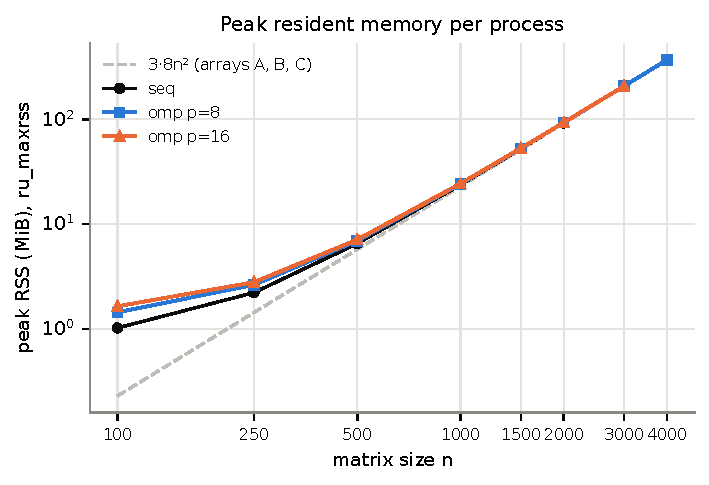
\includegraphics[width=0.55\linewidth]{fig5_memory}
\caption{Peak resident memory per process against $n$; the parallel curves lie on top of the sequential one.}
\label{fig:mem}
\end{figure}

\subsection{Variability between passes and within processes}\label{sec:var}
The second pass at $n=2000$, run ten minutes after the first at the end of the campaign, was \textbf{faster for every configuration, by
2.8--17.3\%} (median $-11\%$; Table~\ref{tab:pass2}, Fig.~\ref{fig:pass2}); it also had smaller IQRs (0.4--2.6\% against 0.9--13\%).
Because sequential and parallel runs moved in the same direction, the speedups changed much less: $S(4)$ from 3.50 to 3.58, $S(8)$ from 3.55 to 3.78,
$S(16)$ from 3.38 to 3.74. The same single-threaded computation at $n=2000$ took 2.64 and 2.68~s in the first pass, 2.42 and 2.38~s in the second,
2.54~s in the tile sweep and 2.42--2.44~s in the vectorisation campaign: the slow interval is the first part of the campaign, not the end, so
the difference is not progressive heating. Its cause could not be identified (no thermal limit was reported and no other application was open).
Within single processes, the longest runs with $p\ge3$ became slower from sample to sample: at $n=3000$ the last sample took 4--8\% longer than the
warm-up and at $n=4000$ 5--6\% longer, while one-thread runs changed by less than 3\% (Table~\ref{tab:drift}). At $n=2000$ (shorter runs) the
changes have both signs ($-7$ to $+8\%$).

\begin{table}[!htb]\centering\footnotesize
\caption{Second pass at $n=2000$: medians (relative IQR), difference pass 2 vs.\ pass 1, and speedups of each pass.}
\label{tab:pass2}\begin{tabular}{llllll}
\toprule
config & pass 1 & pass 2 & $\Delta$ (\%) & $S$ pass 1 & $S$ pass 2 \\
\midrule
seq & 2.64 s (4.2\%) & 2.42 s (2.2\%) & -8.4 & -- & -- \\
$p{=}1$ & 2.68 s (0.89\%) & 2.38 s (2.2\%) & -11.4 & 0.983 & 1.02 \\
$p{=}2$ & 1.41 s (6.4\%) & 1.25 s (0.38\%) & -11.7 & 1.87 & 1.94 \\
$p{=}3$ & 932 ms (8.5\%) & 845 ms (0.46\%) & -9.4 & 2.83 & 2.86 \\
$p{=}4$ & 755 ms (6.2\%) & 675 ms (2.6\%) & -10.6 & 3.50 & 3.58 \\
$p{=}6$ & 729 ms (2.5\%) & 708 ms (1.9\%) & -2.8 & 3.62 & 3.42 \\
$p{=}8$ & 744 ms (13\%) & 640 ms (1.5\%) & -13.9 & 3.55 & 3.78 \\
$p{=}16$ & 782 ms (3.0\%) & 647 ms (1.1\%) & -17.3 & 3.38 & 3.74 \\
\bottomrule
\end{tabular}

\end{table}

\begin{figure}[!htb]\centering
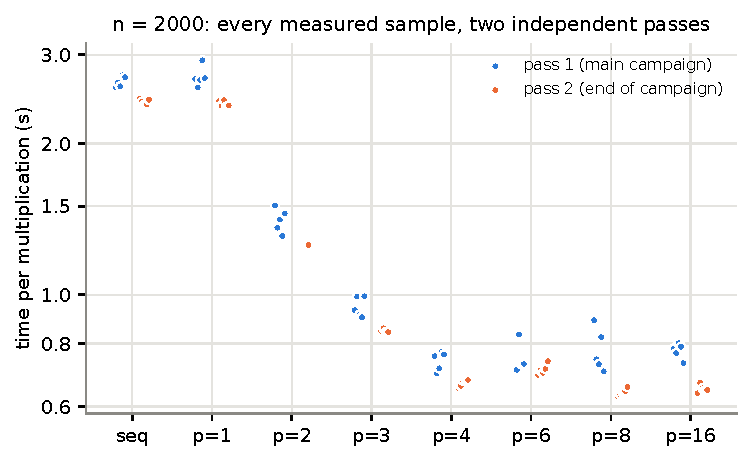
\includegraphics[width=0.6\linewidth]{fig6_pass2}
\caption{Every measured sample at $n=2000$ in the first pass (main campaign) and in the second pass at the end of the campaign.}
\label{fig:pass2}
\end{figure}

\begin{table}[!htb]\centering\footnotesize
\caption{Within-process drift: last measured sample relative to the warm-up sample of the same process (\%), for the longest runs.}
\label{tab:drift}\begin{tabular}{rrrrrrrrr}
\toprule
$n$ & seq & $p{=}1$ & $p{=}2$ & $p{=}3$ & $p{=}4$ & $p{=}6$ & $p{=}8$ & $p{=}16$ \\
\midrule
2000 & +1.2 & -2.9 & +1.9 & -5.8 & +8.4 & +4.0 & -0.0 & -7.2 \\
3000 & -2.2 & -1.6 & +0.8 & +4.2 & +5.1 & +4.5 & +8.3 & +7.2 \\
4000 & -1.0 & +1.4 & -- & -- & +6.2 & -- & +5.2 & -- \\
\bottomrule
\end{tabular}

\end{table}

\subsection{Reference comparisons}
\textbf{Basic algorithm.} The unchanged Assignment~1 i-j-k kernel takes 140~ms at $n=500$ and 1.86~s at $n=1000$: $3.5\times$ and $5.8\times$
slower than the blocked baseline and $13\times$ and $23\times$ slower than the parallel version with 8 threads (Table~\ref{tab:ijk}).
\textbf{Tile size.} The tile $b=96$ was fixed before the campaign from Assignment~2. On this CPU a short check at $n=2000$ found $b=64$ fastest
sequentially (2.26~s vs.\ 2.54~s for $b=96$) and $b=32$ fastest with 4 threads (628 vs.\ 660~ms); $S(4)$ stayed between 3.54 and 3.86 for all five
tiles (Table~\ref{tab:bsweep}, Fig.~\ref{fig:bsweep}).

\begin{table}[!htb]\centering\footnotesize
\begin{minipage}{0.5\linewidth}\centering
\caption{A1 i-j-k reference (sequential).}\label{tab:ijk}\resizebox{\linewidth}{!}{\begin{tabular}{rlllll}
\toprule
$n$ & ijk (A1) & seq (blocked) & omp $p{=}8$ & ijk/seq & ijk/omp$_8$ \\
\midrule
500 & 140 ms (2.9\%) & 40.0 ms & 10.5 ms & 3.49 & 13.3 \\
1000 & 1.86 s (1.6\%) & 320 ms & 81.4 ms & 5.81 & 22.8 \\
\bottomrule
\end{tabular}
}
\end{minipage}\hfill
\begin{minipage}{0.45\linewidth}\centering
\caption{Tile-size check, $n=2000$.}\label{tab:bsweep}\begin{tabular}{rlll}
\toprule
tile $b$ & seq & omp $p{=}4$ & $S(4)$ \\
\midrule
32 & 2.41 s (0.50\%) & 628 ms (0.78\%) & 3.83 \\
64 & 2.26 s (1.0\%) & 638 ms (3.5\%) & 3.54 \\
96 & 2.54 s (0.50\%) & 660 ms (0.66\%) & 3.86 \\
128 & 2.46 s (2.0\%) & 686 ms (1.8\%) & 3.58 \\
192 & 2.60 s (0.54\%) & 710 ms (1.2\%) & 3.66 \\
\bottomrule
\end{tabular}

\end{minipage}
\end{table}

\begin{figure}[!htb]\centering
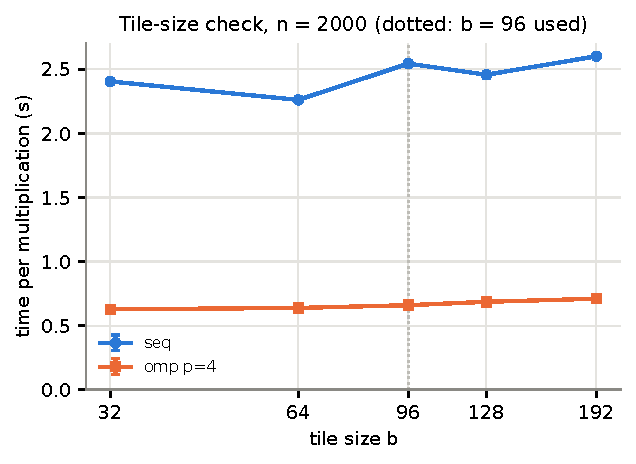
\includegraphics[width=0.48\linewidth]{fig8_bsweep}
\caption{Time per multiplication against the tile size at $n=2000$ (campaign \texttt{bsweep}); error bars are the IQR.}
\label{fig:bsweep}
\end{figure}

\subsection{Supplementary experiment: where parallelism stops paying off}
The 15 processes of the supplementary campaign were all correct, bit-identical to the baseline and without thermal limit. Table~\ref{tab:small}
and Fig.~\ref{fig:small} show the result. At $n=16$, where one sequential multiplication takes 1.47~$\mu$s, \textbf{every parallel configuration
is slower than the baseline}: $S=0.82$, $0.70$, $0.53$ and $0.40$ for $p=1,2,4,8$, i.e.\ more threads make it worse. At $n=32$ (9.6~$\mu$s)
parallel execution already pays: $S(2)=1.70$, $S(4)=2.56$ (noisy: relative IQR 38\%, IQR-based range 1.86--2.58), $S(8)=2.06$; at $n=64$
(70~$\mu$s) $S(4)=2.95$. The break-even therefore lies between $n=16$ and $n=32$ for this machine and timing boundary. For $n\le64$, 8 threads
are always slower than 4. Assuming the work itself divides perfectly, $T_p-T_{seq}/p$ at $n=16$ estimates the cost of one parallel region:
0.33~$\mu$s with one thread, 1.4, 2.4 and 3.5~$\mu$s with 2, 4 and 8 threads.

\begin{table}[!htb]\centering\footnotesize
\caption{Supplementary campaign \texttt{small} (added after the main results): median time per multiplication (relative IQR for \texttt{seq}) and [speedup $S(p)$].}
\label{tab:small}\begin{tabular}{rlllll}
\toprule
$n$ & seq & $p{=}1$ & $p{=}2$ & $p{=}4$ & $p{=}8$ \\
\midrule
16 & 1.47 $\mu$s (5.9\%) & 1.80 $\mu$s [0.82] & 2.11 $\mu$s [0.70] & 2.77 $\mu$s [0.53] & 3.65 $\mu$s [0.40] \\
32 & 9.58 $\mu$s (0.77\%) & 10.0 $\mu$s [0.95] & 5.63 $\mu$s [1.70] & 3.74 $\mu$s [2.56] & 4.65 $\mu$s [2.06] \\
64 & 69.6 $\mu$s (1.1\%) & 69.8 $\mu$s [1.00] & 37.2 $\mu$s [1.87] & 23.6 $\mu$s [2.95] & 26.7 $\mu$s [2.60] \\
\bottomrule
\end{tabular}

\end{table}

\begin{figure}[!htb]\centering
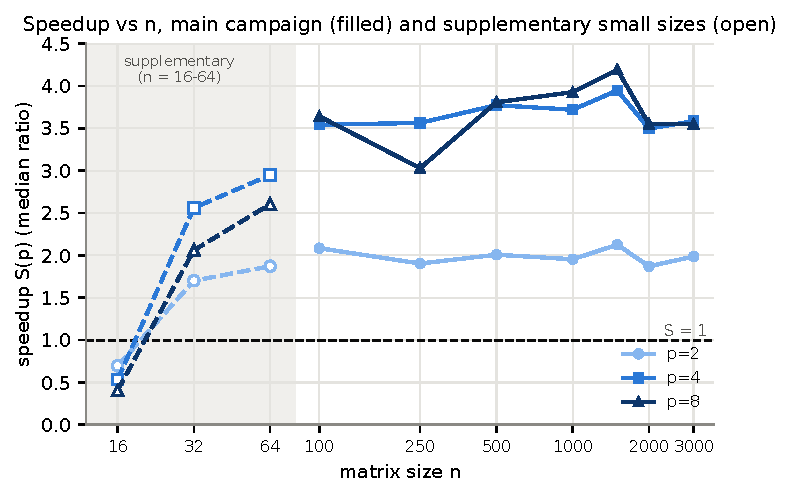
\includegraphics[width=0.62\linewidth]{fig9_small}
\caption{Speedup against $n$ including the supplementary sizes $n=16$--$64$ (open markers, separate later campaign; shaded) and the main campaign (filled). Below the horizontal line the parallel version is slower than the baseline.}
\label{fig:small}
\end{figure}

\subsection{Optional extension: vectorisation}
\textbf{Evidence.} Clang reports the inner $j$ loop of the kernel (line 101) as ``not vectorized'' in the scalar build, ``vectorized loop
(vectorization width: 2, interleaved count: 2)'' with SSE2 and ``(vectorization width: 4, interleaved count: 4)'' with AVX2. The disassembly of the
kernel agrees (Table~\ref{tab:vecev}): the scalar build contains only scalar \texttt{mulsd}/\texttt{addsd}, the SSE2 build packed \texttt{mulpd}/\texttt{addpd}
on 128-bit \texttt{xmm} registers, and the AVX2 build \texttt{vmulpd}/\texttt{vaddpd} on 256-bit \texttt{ymm} registers; no build contains FMA
instructions. One scalar multiply and one scalar add remain in each build (in the vector builds, presumably the remainder iterations of the loop).

\begin{table}[!htb]\centering\footnotesize\setlength{\tabcolsep}{4pt}
\caption{Vectorisation evidence: instruction counts in the disassembly of \texttt{mul\_blocked\_rows} (\texttt{otool -tv}) and clang remark for the inner loop.}
\label{tab:vecev}\resizebox{\linewidth}{!}{\begin{tabular}{llrrrrrl}
\toprule
build & extra flags & mulpd & addpd & mulsd & addsd & ymm & compiler remark (inner loop) \\
\midrule
scalar & \texttt{-fno-vectorize -fno-slp-vectorize} & 0 & 0 & 1 & 1 & 0 & \parbox[t]{5.2cm}{\raggedright\footnotesize loop not vectorized} \\
sse2 & -- & 6 & 6 & 1 & 1 & 0 & \parbox[t]{5.2cm}{\raggedright\footnotesize vectorized loop (vectorization width: 2, interleaved count: 2)} \\
avx2 & \texttt{-mavx2} & 4 & 4 & 1 & 1 & 13 & \parbox[t]{5.2cm}{\raggedright\footnotesize vectorized loop (vectorization width: 4, interleaved count: 4)} \\
\bottomrule
\end{tabular}
}
\end{table}

\textbf{Performance.} Table~\ref{tab:vec} and Fig.~\ref{fig:vec} cross the three builds with the thread counts. The bracketed factor is the
\emph{SIMD gain} $T_{scalar}(p)/T_{build}(p)$ at the same $p$ and $n$, so it isolates code generation from thread count. SSE2 is 2.23--2.88$\times$
faster than scalar code and AVX2 3.94--5.08$\times$ faster, at every $p$. Within each build, the thread speedup at $p=4$ is 3.09--3.56 (scalar),
3.61--3.89 (SSE2) and 3.38--3.56 (AVX2). Going from 4 to 8 threads raises the throughput of the scalar build at $n=1000$ by 23\% (235 to 192~ms) but slightly
slows the AVX2 build (46.2 to 48.6~ms at $n=1000$, 364 to 378~ms at $n=2000$). At $n=2000$ the AVX2 gain decreases from 4.40 (sequential) to
4.01 ($p=8$); at $n=1000$ it does not decrease monotonically (5.08 at $p=4$). The fastest configuration, AVX2 with 4 threads, reaches
43.9~GFLOP/s at $n=2000$, $14.9\times$ the scalar sequential time. All 30 products were bit-identical to the baseline.

\begin{table}[!htb]\centering\footnotesize
\caption{Vectorisation $\times$ threads (campaign \texttt{vec}): median time and [SIMD gain $T_{scalar}(p)/T(p)$]. The SSE2 build is byte-identical to the primary binary.}
\label{tab:vec}\resizebox{0.9\linewidth}{!}{\begin{tabular}{rllllll}
\toprule
$n$ & build & seq & $p{=}1$ & $p{=}2$ & $p{=}4$ & $p{=}8$ \\
\midrule
1000 & scalar & 726 ms [1.00] & 714 ms [1.00] & 371 ms [1.00] & 235 ms [1.00] & 192 ms [1.00] \\
1000 & SSE2, 128-bit & 317 ms [2.29] & 306 ms [2.33] & 161 ms [2.30] & 81.6 ms [2.88] & 80.2 ms [2.39] \\
1000 & AVX2, 256-bit & 165 ms [4.41] & 168 ms [4.25] & 84.8 ms [4.37] & 46.2 ms [5.08] & 48.6 ms [3.94] \\
\midrule
2000 & scalar & 5.42 s [1.00] & 5.45 s [1.00] & 2.83 s [1.00] & 1.52 s [1.00] & 1.52 s [1.00] \\
2000 & SSE2, 128-bit & 2.42 s [2.24] & 2.44 s [2.24] & 1.25 s [2.26] & 669 ms [2.28] & 679 ms [2.23] \\
2000 & AVX2, 256-bit & 1.23 s [4.40] & 1.23 s [4.42] & 646 ms [4.37] & 364 ms [4.18] & 378 ms [4.01] \\
\bottomrule
\end{tabular}
}
\end{table}

\begin{figure}[!htb]\centering
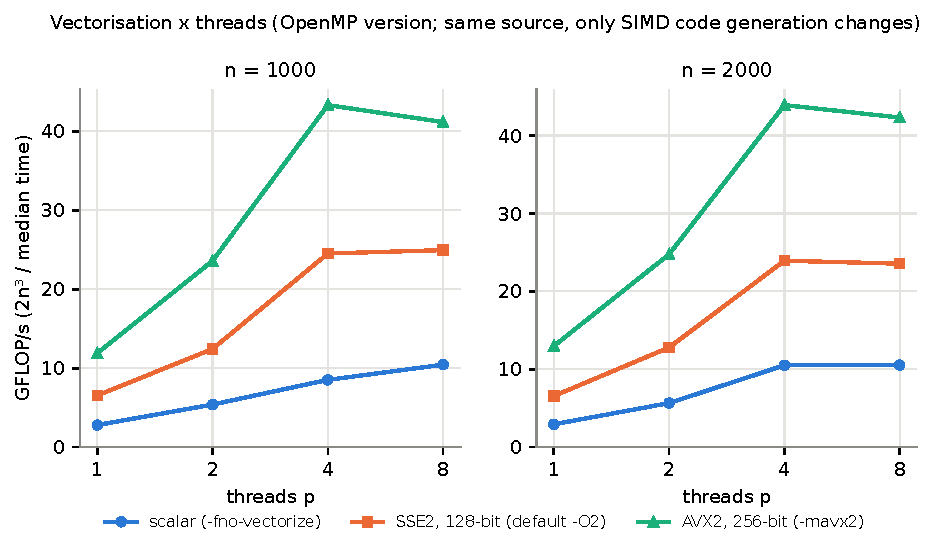
\includegraphics[width=0.85\linewidth]{fig7_vec}
\caption{Throughput ($2n^3$/median time) of the parallel version for the three builds; vertical distance between curves = SIMD effect at fixed $p$, slope of each curve = thread effect for a fixed build.}
\label{fig:vec}
\end{figure}
